\documentclass[compress]{beamer}

\usetheme{Madrid}
\useoutertheme{miniframes} % Alternatively: miniframes, infolines, split
\useinnertheme{circles}

%\setbeamertemplate{background} 
%{
%	\includegraphics[width=0.8\textwidth]{img/background-kiv.pdf}
%}

%\definecolor{UBCblue}{rgb}{0.04706, 0.13725, 0.26667} % UBC Blue (primary)
\definecolor{UBCblue}{rgb}{0.04706, 0.13725, 0.26667} % UBC Blue (primary)
\definecolor{UBCgrey}{rgb}{0.3686, 0.5255, 0.6235} % UBC Grey (secondary)

\setbeamercolor{palette primary}{bg=UBCblue,fg=white}
\setbeamercolor{palette secondary}{bg=UBCblue,fg=white}
\setbeamercolor{palette tertiary}{bg=UBCblue,fg=white}
\setbeamercolor{palette quaternary}{bg=UBCblue,fg=white}
\setbeamercolor{structure}{fg=UBCblue} % itemize, enumerate, etc
\setbeamercolor{section in toc}{fg=UBCblue} % TOC sections

% Override palette coloring with secondary
\setbeamercolor{subsection in head/foot}{bg=UBCgrey,fg=white}
\setbeamertemplate{caption}[numbered]
\setbeamercovered{transparent}

\usepackage{xcolor}
\usepackage{fontspec}
\usefonttheme{serif}

\title[Rpi Zero emulátor]{Emulátor ARMv6 procesoru \\ pro emulaci prostředí Raspberry Pi}
\date{17. 06. 2024}
\author[Jakub Šilhavý]{Bc. Jakub Šilhavý}
\institute[KIV ZČU]{vedoucí práce: Ing. Martin Úbl \\ \bigskip Katedra informatiky a výpočetní techniky \\ Fakulta aplikovaných věd \\ Západočeská univerzita v Plzni}

\begin{document}
	
\begin{frame}
    \titlepage
\end{frame}

\section{Zadání práce}

\subsection{Cíl práce}

\begin{frame}
	\begin{block}{Cíl práce}
		\begin{itemize}
			\item návrh a implementace emulátoru platformy \textbf{Raspberry Pi Zero}
			\begin{itemize}
				\item<2-> emulace instrukcí procesoru \texttt{ARM1176JZF-S} (\texttt{ARMv6})
				\item<3-> emulace základních periferií \texttt{µC} \texttt{BCM2835} (\texttt{GPIO}, \texttt{Mini\_UART}, \texttt{BSC}, ...)
			\end{itemize}
		\end{itemize}
	\end{block}
	\begin{columns}
		\column{0.57\textwidth}
		\begin{enumerate}
			\item<4-> vzdělávací účely
			\begin{itemize}
				\item<4-> vizualizace principů \texttt{OS}
				\item<4-> embedded vývoj
			\end{itemize}
			\item<5-> testování a ladění \texttt{SW}
			\item<6-> prototypování \texttt{HW}
			\begin{itemize}
				\item<6-> připojení externích periferií
				\item<6-> návrh vlastního systému
			\end{itemize}
		\end{enumerate}
		\column{0.4\textwidth}
		\begin{figure}
			\centering
			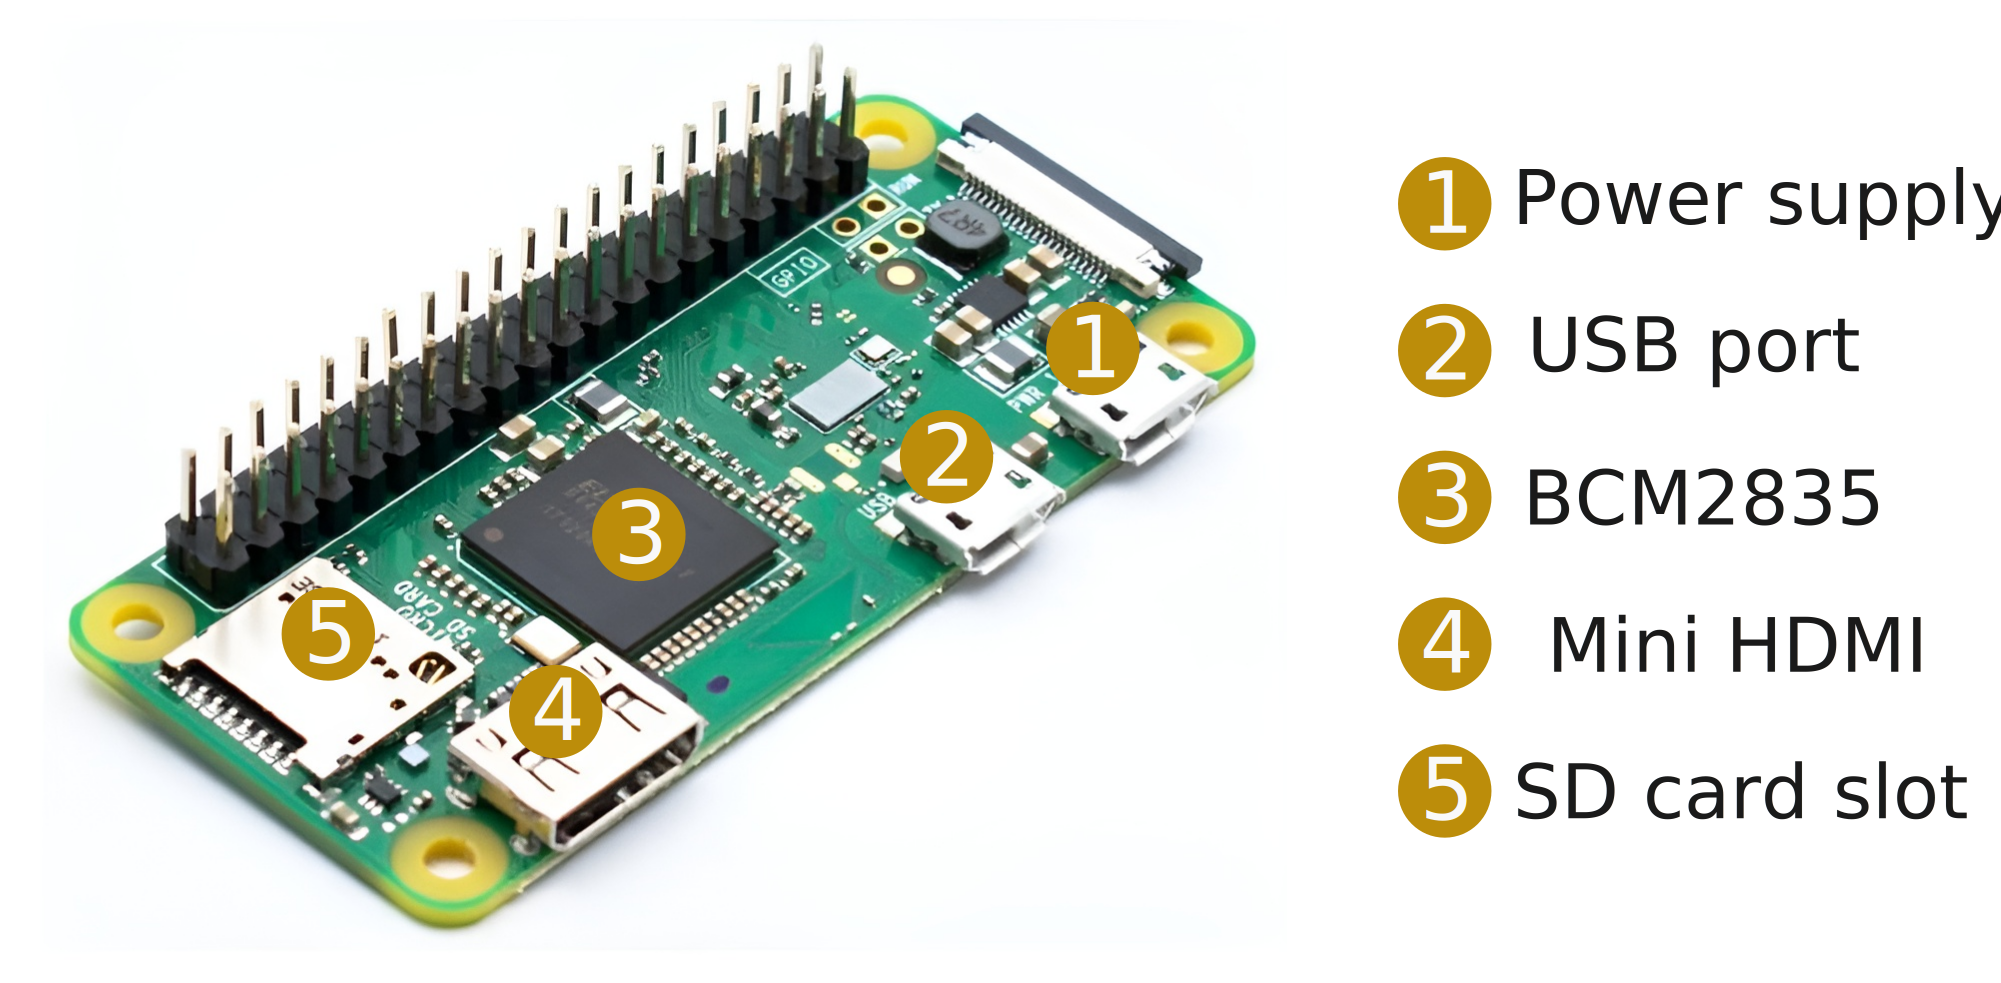
\includegraphics[width=0.60\textwidth]{img/rpi_zero.jpeg}
			\caption{Raspberry Pi Zero}
			\label{Raspberry Pi Zero}
		\end{figure}
	\end{columns}
	\vspace{0.2cm}
	\noindent\makebox[\linewidth]{\rule{\textwidth}{0.4pt}}
	\vspace{-0.4cm}
	\begin{itemize}
		\item<7-> použití \href{https://github.com/MartinUbl/KIV-RTOS}{\beamergotobutton{KIV-RTOS}} pro ověření správnosti výsledného emulátoru
	\end{itemize}
\end{frame}

\subsection{\texttt{ARMv6} aplikace}

\begin{frame}
	\begin{columns}
		\column{0.45\textwidth}
			\begin{figure}
			\centering
			\includegraphics[width=0.85\textwidth]{img/arm_powered_products.jpg}
			\caption{\texttt{ARM} aplikace}
			\label{ARM aplikace}
		\end{figure}
		\column{0.55\textwidth}
			\begin{figure}
			\centering
			\includegraphics[width=0.9\textwidth]{img/arm_processor_roadmap2.jpeg}
			\caption{\texttt{ARM} \texttt{CPU} roadmap}
			\label{ARM CPU roadmap}
		\end{figure}
	\end{columns}
\end{frame}

\section{Existující řešení}

\subsection{CPUlator, ARMSim\#}

\begin{frame}
	\begin{columns}
		\column{0.5\textwidth}
		\begin{itemize}
			\item vhodné pro seznámení se s programování v \texttt{JSA}
			\begin{itemize}
				\item vizualizace, ladění programu
			\end{itemize}
			\item floating-point instrukce
			\item platformová nezávislost
		\end{itemize}
		\column{0.5\textwidth}
		\begin{figure}
			\centering
			\includegraphics[width=0.8\textwidth]{img/cpulator.png}
			\caption{\href{https://cpulator.01xz.net}{\beamergotobutton{CPUlator}}}
			\label{CPUlator}
		\end{figure}
	\end{columns}
	\noindent\makebox[\linewidth]{\rule{\textwidth}{0.4pt}}
	\begin{block}{Omezení}
		\begin{itemize}
			\item emulace pouze \texttt{CPU} (ne celého \texttt{SoC})
			\item minimální podpora pokročilých systémových operací
			\begin{itemize}
				\item $\Rightarrow$ nevhodné pro testování pricipů \texttt{OS}
			\end{itemize}
			\item limitovaná podpora připojení externích periferií
		\end{itemize}
	\end{block}
\end{frame}

\subsection{QEMU}

\begin{frame}
	\begin{columns}
		\column{0.6\textwidth}
		\begin{itemize}
			\item podpora různých architektur
			\begin{itemize}
				\item \texttt{x86}, \texttt{MIPS}, \texttt{ARM}, ...
			\end{itemize}
			\item připojení externího debuggeru
			\item plná podpora systémových oprací
		\end{itemize}
		\column{0.4\textwidth}
		\begin{figure}
			\centering
			\includegraphics[width=0.6\textwidth]{img/Qemu_logo.pdf}
			\caption{\href{https://www.qemu.org}{\beamergotobutton{QEMU}}}
			\label{QEMU}
		\end{figure}
	\end{columns}
	\vspace{0.4cm}
	\noindent\makebox[\linewidth]{\rule{\textwidth}{0.4pt}}
	\begin{block}{Omezení}
		\begin{itemize}
			\item emulace pouze \texttt{CPU} (ne celého \texttt{SoC})
			\item limitovaná podpora připojení externích periferií
			\item \texttt{\_start} symbol očekáván na adrese \texttt{0x00010000} (\texttt{ARM})
			\begin{itemize}
				\item $\Rightarrow$ nekompatibilita s \textit{first-stage} \texttt{BL} \texttt{Rpi0} (\texttt{0x00008000})
			\end{itemize}
			\item problémy se \texttt{systimer}
		\end{itemize}
	\end{block}
\end{frame}

\section{ZeroMate}

\subsection{Jádro emulátoru}

\begin{frame}
	\begin{columns}
		\column{0.4\textwidth}
		\begin{block}{\texttt{ARM1176JZF-S}}
			\begin{itemize}
				\item \texttt{ARMv6} instrukce
				\item přepínání režimů \texttt{CPU}
				\item \texttt{ALU}, \texttt{MAC} a \texttt{MMU}
				\item vyjímky a přerušení
				\item podpora ko-procesorů
				\begin{itemize}
					\item \texttt{CP15}, \texttt{CP10}
				\end{itemize}
				\item systémová sběrnice
			\end{itemize}
		\end{block}
		\column{0.4\textwidth}
		\begin{block}{\texttt{BCM2835}}
			\begin{itemize}
				\item \texttt{RAM}
				\item interrupt controller
				\item \texttt{ARM} timer
				\item \texttt{TRNG}
				\item \texttt{GPIO}
				\item \texttt{BSC\_1} (\texttt{I\textsuperscript{2}C})
				\item \texttt{AUX} (\texttt{Mini\_UART})
				\item debug monitor* 
			\end{itemize}
		\end{block}
	\end{columns}
	\vspace{0.4cm}
	\noindent\makebox[\linewidth]{\rule{\textwidth}{0.4pt}}
	\vspace{-0.4cm}
	\begin{itemize}
		\item cílem bylo emulovat nejčastěji používané periferie
		\item dekompoziční návrh architektury 
		\begin{itemize}
			\item $\Rightarrow$ snadné rozšíření o další periferie
		\end{itemize}
	\end{itemize}
\end{frame}

\subsection{Externí periferie}

\begin{frame}
	\vspace{0.4cm}
	\begin{itemize}
		\item jednotné rozhraní pro externí periferie (připojeny přes \texttt{GPIO})
		\item načtené při inicializaci jako sdílené knihovny (\texttt{.dll}, \texttt{.so})
		\begin{itemize}
			\item možnost načtení vícero instancí (např. \texttt{led.dll})
		\end{itemize}
		\item nezávislé na toolchainu jádra emulátoru
	\end{itemize}
	\begin{figure}
		\centering
		\includegraphics[width=0.6\textwidth]{img/peripheral_interface.pdf}
		\caption{Rozhraní externích periferií}
	\end{figure}
\end{frame}

\section{Ukázka}

\subsection{ZeroMate - uživatelské rozhraní}

\begin{frame}
	\centering \Large
	\begin{overlayarea}{\textwidth}{\textheight}
		\begin{figure}
			\centering
			\only<1>
			{%
				\includegraphics[width=.85\textwidth]{img/gui/01.pdf}%
			}%
			\only<2>
			{%
				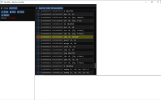
\includegraphics[width=.85\textwidth]{img/gui/02.pdf}%
			}%
			\only<3>
			{%
				\includegraphics[width=.85\textwidth]{img/gui/03.pdf}%
			}%
			\only<4>
			{%
				\includegraphics[width=.85\textwidth]{img/gui/04.pdf}%
			}%
			\only<5>
			{%
				\includegraphics[width=.85\textwidth]{img/gui/05.pdf}%
			}%
		\end{figure}
	\end{overlayarea}      
\end{frame}

\subsection{ZeroMate - externí periferie}

\begin{frame}
	\centering \Large
	\begin{overlayarea}{\textwidth}{\textheight}
		\begin{figure}
			\centering
			\only<1>
			{%
				\includegraphics[width=.85\textwidth]{img/screenshot-02.pdf}%
			}%
			\only<2>
			{%
				\includegraphics[width=.85\textwidth]{img/screenshot-03.pdf}%
			}%
			\only<3>
			{%
				\includegraphics[width=.85\textwidth]{img/screenshot-04.pdf}%
			}%
			\only<4>
			{%
				\includegraphics[width=.85\textwidth]{img/screenshot-05.pdf}%
			}%
			\only<5>
			{%
				\includegraphics[width=.85\textwidth]{img/screenshot-06.pdf}%
			}%
			\only<6>
			{%
				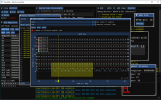
\includegraphics[width=.85\textwidth]{img/screenshot-07.pdf}%
			}%
		\end{figure}
	\end{overlayarea}      
\end{frame}

\section{Technlogie}

\begin{frame}
	\vspace{-0.5cm}
	\begin{figure}
		\centering
		\includegraphics[width=0.07\textwidth]{img/logos/github.pdf}
	\end{figure}
	\centering
	\vspace{-0.4cm}
	\href{https://github.com/silhavyj/ZeroMate}{\beamergotobutton{https://github.com/silhavyj/ZeroMate}}
	\vspace{-0.1cm}
	\noindent\makebox[\linewidth]{\rule{\textwidth}{0.4pt}}
	\begin{figure}
		\centering
		
\includegraphics[width=0.7\textwidth]{img/logos/logos.pdf}
	\end{figure}
	\begin{itemize}
		\item \texttt{OpenGL} jako jediná závislost
			\begin{itemize}
				\item zbytek automaticky stažen a sestaven (\texttt{.gitmodules} + \texttt{CMake})
			\end{itemize}
	\end{itemize}
\end{frame}

\section{Závěr}

\begin{frame}
  \centering \Large
  Děkuji Vám za pozornost\\
  \href{https://github.com/silhavyj/ZeroMate}{\beamergotobutton{https://github.com/silhavyj/ZeroMate}}
  \begin{figure}
  	\centering
  	\includegraphics[width=0.10\textwidth]{img/qr-code.pdf}
  \end{figure}
\end{frame}

\end{document}